\documentclass[10pt,a4paper]{article}
\usepackage[margin=22mm]{geometry}
\usepackage[T1]{fontenc}
\usepackage{lmodern,amsmath,amssymb,booktabs,graphicx,tikz,hyperref,fvextra}
\usetikzlibrary{arrows.meta,positioning,calc,decorations.pathmorphing}
\definecolor{ink}{RGB}{20,53,78}
\hypersetup{colorlinks=true,urlcolor=ink,linkcolor=ink}
\setlength{\parindent}{0pt}
\setlength{\parskip}{5pt}
\emergencystretch=3em

\title{\color{ink}Flywheel speed regulation under a load torque}
\author{}
\date{Original learning collection -- November 2026}
\begin{document}
\begin{center}{\LARGE\color{ink}Flywheel speed regulation under a load torque}\\[5pt]{\small Original learning collection -- November 2026}\end{center}

\textbf{Evidence note.} Original teaching scenario. Numerical parameters are deliberately chosen for learning. All generated data and curves are synthetic; no physical measurement is asserted.
\section{Design brief}
A synthetic DC motor drives a flywheel with $R=2\,\Omega$, $L=0.02\,\mathrm{H}$, $J=0.01\,\mathrm{kg\,m^2}$, $b=0.02\,\mathrm{N\,m\,s/rad}$ and $k_t=k_e=0.1$ in consistent SI units. Derive the voltage-to-speed and opposing-load-to-speed transfers. Compare proportional gain $k_p=0.8$ with PI gains $k_p=0.8$, $k_i=1.6$ for reference $5\,\mathrm{rad/s}$ and load $0.03\,\mathrm{N\,m}$ applied at $t=4\,\mathrm{s}$. Explain the benefits and limits of integral action.
\section{Physical system}
\begin{center}\resizebox{\ifdim\width>.98\linewidth.98\linewidth\else\width\fi}{!}{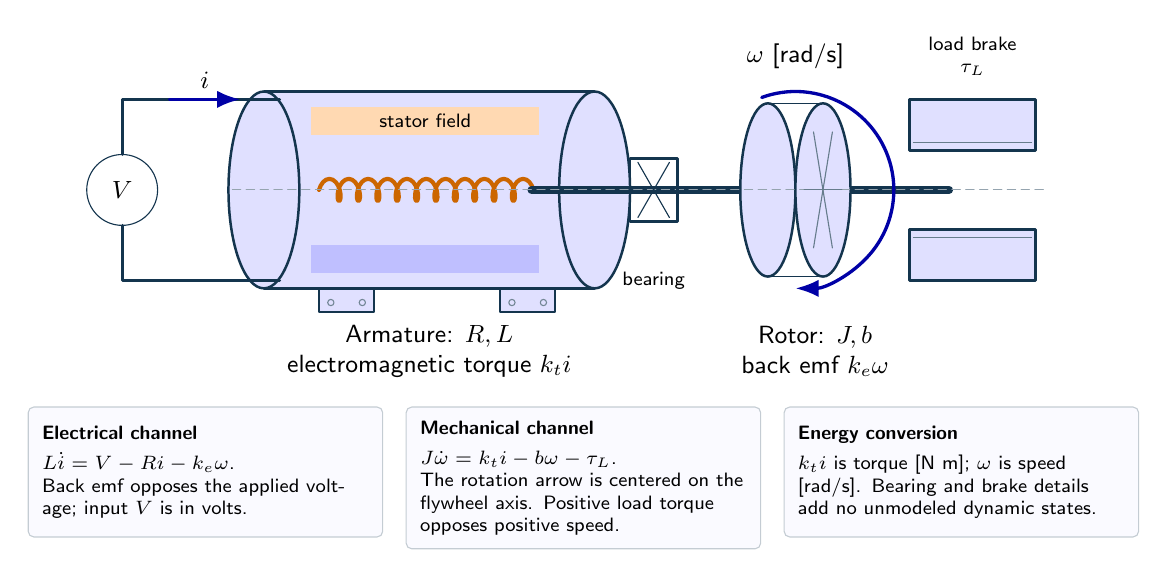
\begin{tikzpicture}[
font=\sffamily\small,>=Latex,line cap=round,line join=round,
wall/.style={draw=ink,line width=1.2pt,fill=blue!5},
water/.style={fill=cyan!25,draw=none},
metal/.style={draw=ink,fill=blue!12,line width=.9pt},
flow/.style={->,draw=blue!65!black,line width=1.2pt},
heat/.style={->,draw=orange!85!black,line width=1.1pt},
measure/.style={->,draw=teal!70!black,line width=.9pt},
dim/.style={<->,draw=ink!65,line width=.6pt},
spring/.style={draw=ink,decorate,decoration={coil,aspect=.5,segment length=4pt,amplitude=3pt}},
wire/.style={draw=ink,line width=1pt},
lab/.style={align=center,font=\sffamily\small},
smalllab/.style={align=center,font=\sffamily\scriptsize}]

\draw[metal](3,1.4)rectangle(7.2,3.9);
\draw[metal](3,2.65)ellipse(.45 and 1.25);
\draw[metal](7.2,2.65)ellipse(.45 and 1.25);
\fill[orange!30](3.6,3.35)rectangle(6.5,3.7);
\fill[blue!25](3.6,1.6)rectangle(6.5,1.95);
\node[smalllab]at(5.05,3.53){stator field};
\draw[orange!80!black,line width=1.5pt,decorate,decoration={coil,segment length=7pt,amplitude=4pt}](3.7,2.65)--(6.5,2.65);
\draw[ink,line width=3pt](6.4,2.65)--(11.7,2.65);
\draw[metal](9.4,2.65)ellipse(.35 and 1.1);
\draw[metal](10.1,2.65)ellipse(.35 and 1.1);
\draw[ink](9.4,3.75)--(10.1,3.75)(9.4,1.55)--(10.1,1.55);
\draw[metal](11.2,1.5)rectangle(12.8,2.15);
\draw[metal](11.2,3.15)rectangle(12.8,3.8);
\node[smalllab]at(12,4.35){load brake\\$\tau_L$};
\draw[flow]($(9.75,2.65)+(110:1.25)$)arc[start angle=110,end angle=-90,radius=1.25];
\node[lab]at(9.75,4.35){$\omega$ [rad/s]};
\draw[wire](3.2,3.8)--(1.2,3.8)--(1.2,3.1)(3.2,1.5)--(1.2,1.5)--(1.2,2.2);
\draw[ink](1.2,2.65)circle(.45);
\node at(1.2,2.65){$V$};
\draw[flow](1.8,3.8)--(2.7,3.8)node[midway,above]{$i$};
\node[lab]at(5.1,.6){Armature: $R,L$\\electromagnetic torque $k_t i$};
\node[lab]at(10,.6){Rotor: $J,b$\\back emf $k_e\omega$};
% REFINED EQUIPMENT DETAILS

% Motor feet, bearing blocks, shaft centerline and flywheel spokes.
\draw[metal](3.7,1.1)rectangle(4.4,1.4);\draw[metal](6,1.1)rectangle(6.7,1.4);
\foreach \x in {3.85,4.25,6.15,6.55}{\draw[ink!60](\x,1.22)circle(.04);}
\draw[ink!45,densely dashed](2.6,2.65)--(12.9,2.65);
\draw[metal,fill=none](7.65,2.25)rectangle(8.25,3.05);
\draw[ink](7.75,2.3)--(8.15,3)(7.75,3)--(8.15,2.3);
\foreach \a in {0,60,...,300}{\draw[ink!65](10.1,2.65)--++({.24*cos(\a)},{.85*sin(\a)});}
\draw[ink!65](11.25,3.25)--(12.75,3.25)(11.25,2.05)--(12.75,2.05);
\node[smalllab]at(7.95,1.5){bearing};

\node[draw=ink!25,fill=blue!2,rounded corners=2pt,anchor=north west,text width=4.15cm,minimum height=1.65cm,inner sep=5pt,align=left,font=\sffamily\scriptsize]at(0.0,-0.1){\textbf{Electrical channel}\\[3pt]$L\dot i=V-Ri-k_e\omega$.\\Back emf opposes the applied voltage; input $V$ is in volts.};
\node[draw=ink!25,fill=blue!2,rounded corners=2pt,anchor=north west,text width=4.15cm,minimum height=1.65cm,inner sep=5pt,align=left,font=\sffamily\scriptsize]at(4.8,-0.1){\textbf{Mechanical channel}\\[3pt]$J\dot\omega=k_ti-b\omega-\tau_L$.\\The rotation arrow is centered on the flywheel axis. Positive load torque opposes positive speed.};
\node[draw=ink!25,fill=blue!2,rounded corners=2pt,anchor=north west,text width=4.15cm,minimum height=1.65cm,inner sep=5pt,align=left,font=\sffamily\scriptsize]at(9.6,-0.1){\textbf{Energy conversion}\\[3pt]$k_ti$ is torque [N m]; $\omega$ is speed [rad/s]. Bearing and brake details add no unmodeled dynamic states.};
\end{tikzpicture}
}\par{\small A voltage-driven motor converts armature current into shaft torque. The rotor and external brake introduce inertia, friction and load torque. The illustrative cutaway does not add magnetic saturation or friction to the stated linear model.}\end{center}
\section{Electromechanical balance}
Let $i$ be armature current, $\omega$ angular speed, $v$ voltage and $d$ opposing load torque. The equations are
\[L\dot i=v-Ri-k_e\omega,\qquad J\dot\omega=k_t i-b\omega-d.\]
Eliminating current yields the common denominator $D(s)=(Ls+R)(Js+b)+k_tk_e$ and
\[G_v(s)=\frac{k_t}{D(s)},\qquad G_d(s)=-\frac{Ls+R}{D(s)}.\]
Numerically $D(s)=0.0002s^2+0.0204s+0.05$ and $G_v(0)=2$ (rad/s)/V.
\section{Closed-loop paths}
For $v=C(s)(r-\omega)$, superposition gives
\[\Omega=\frac{C G_v}{1+C G_v}R+\frac{G_d}{1+C G_v}D_{load}.\]
With proportional control, the final speed is $(K_pG_v(0)r+G_d(0)d)/(1+K_pG_v(0))$. Substitution gives $(8-1.2)/2.6=2.61538$ rad/s after the load arrives.
\section{Integral action and stability}
For $C=0.8+1.6/s$, the characteristic polynomial is
\[0.0002s^3+0.0204s^2+0.13s+0.16.\]
Its positive coefficients satisfy $0.0204(0.13)>0.0002(0.16)$, so the cubic is Hurwitz. A stable loop with integral action rejects a constant load and tracks the constant reference in this ideal unsaturated model. The required steady voltage is not zero: equilibrium requires $i=(br+d)/k_t=1.3$ A and $v=Ri+k_er=3.1$ V.
\section{Limits}
Voltage and current limits, magnetic saturation, brush friction, heating and sensor noise are omitted. Integral action cannot provide an unavailable actuator voltage.
\section{What to learn from the experiment}
Track the disturbance entry point as carefully as the reference path. Zero ideal steady error is conditional on stability and actuator feasibility.
\section{System sketch}
\begin{center}\resizebox{\ifdim\width>.98\linewidth.98\linewidth\else\width\fi}{!}{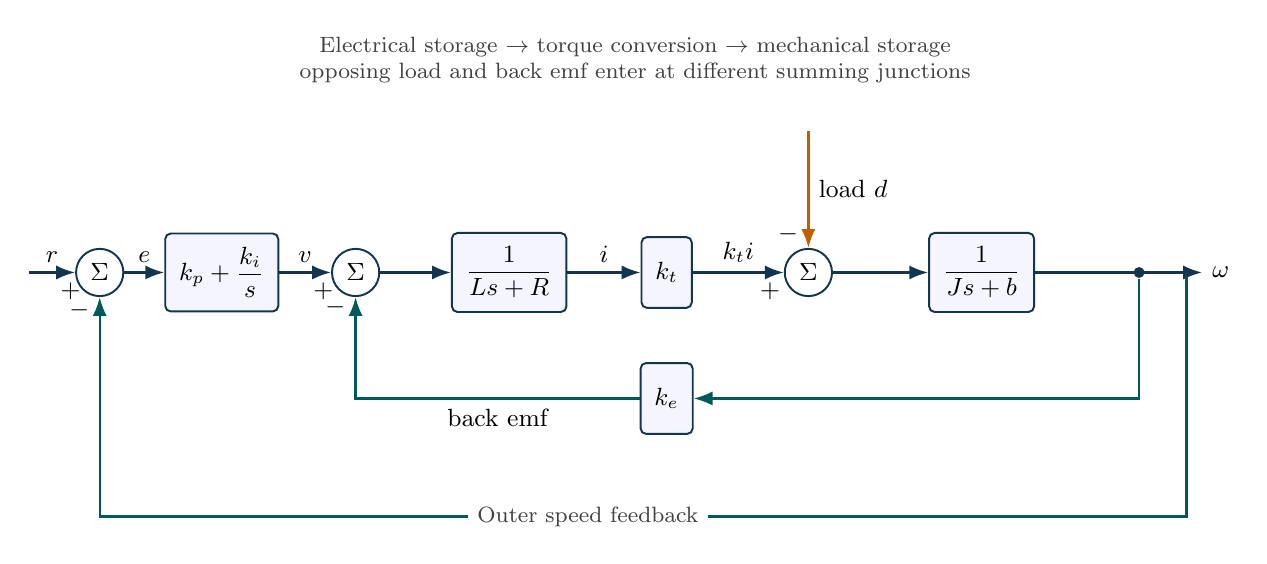
\begin{tikzpicture}[x=1cm,y=1cm,>=Latex,font=\small,
block/.style={draw=ink,fill=blue!4,rounded corners=2pt,minimum height=9mm,align=center,line width=.7pt,inner sep=5pt},
sum/.style={circle,draw=ink,fill=white,minimum size=6mm,inner sep=0pt,line width=.7pt},
sig/.style={->,draw=ink,line width=.85pt},
fb/.style={->,draw=teal!70!black,line width=.85pt},
dist/.style={->,draw=orange!75!black,line width=.85pt},
tap/.style={circle,fill=ink,inner sep=1.4pt},
note/.style={font=\footnotesize,align=center,text=black!75}]

\node[sum](e)at(.8,0){$\Sigma$};
\node[block](c)at(2.35,0){$k_p+\dfrac{k_i}{s}$};
\node[sum](v)at(4.05,0){$\Sigma$};
\node[block](el)at(6,0){$\dfrac{1}{Ls+R}$};
\node[block](kt)at(8,0){$k_t$};
\node[sum](tau)at(9.8,0){$\Sigma$};
\node[block](mech)at(12,0){$\dfrac{1}{Js+b}$};
\node[tap](w)at(14,0){};
\draw[sig](-.1,0)--node[above]{$r$}node[pos=.9,below]{$+$}(e);
\draw[sig](e)--node[above]{$e$}(c);
\draw[sig](c)--node[above]{$v$}node[pos=.85,below]{$+$}(v);
\draw[sig](v)--(el);
\draw[sig](el)--node[above]{$i$}(kt);
\draw[sig](kt)--node[above]{$k_ti$}node[pos=.85,below]{$+$}(tau);
\draw[sig](tau)--(mech);
\draw[sig](mech)--(14.8,0)node[right]{$\omega$};
\draw[dist](9.8,1.8)--node[right]{load $d$}node[pos=.88,left]{$-$}(tau);
\node[block](ke)at(8,-1.6){$k_e$};
\draw[fb](w)--(14,-1.6)--(ke);
\draw[fb](ke)--node[below]{back emf}(4.05,-1.6)--node[pos=.9,left]{$-$}(v);
\draw[fb](14.6,0)--(14.6,-3.1)--(.8,-3.1)--node[pos=.94,left]{$-$}(e);
\fill[ink](14.6,0)circle(1.4pt);
\node[note,fill=white]at(7,-3.1){Outer speed feedback};
\node[note]at(7.6,2.7){Electrical storage $\rightarrow$ torque conversion $\rightarrow$ mechanical storage\\opposing load and back emf enter at different summing junctions};

\end{tikzpicture}
}
\par\small\refstepcounter{figure}\label{fig:system}\textbf{Figure \thefigure.} Outer PI speed regulation around the electromechanical motor. The inner back-emf path and opposing load torque have explicit negative signs.\end{center}
\section{Executed computational evidence}
\VerbatimInput[fontsize=\small,breaklines=true]{results.txt}
\begin{center}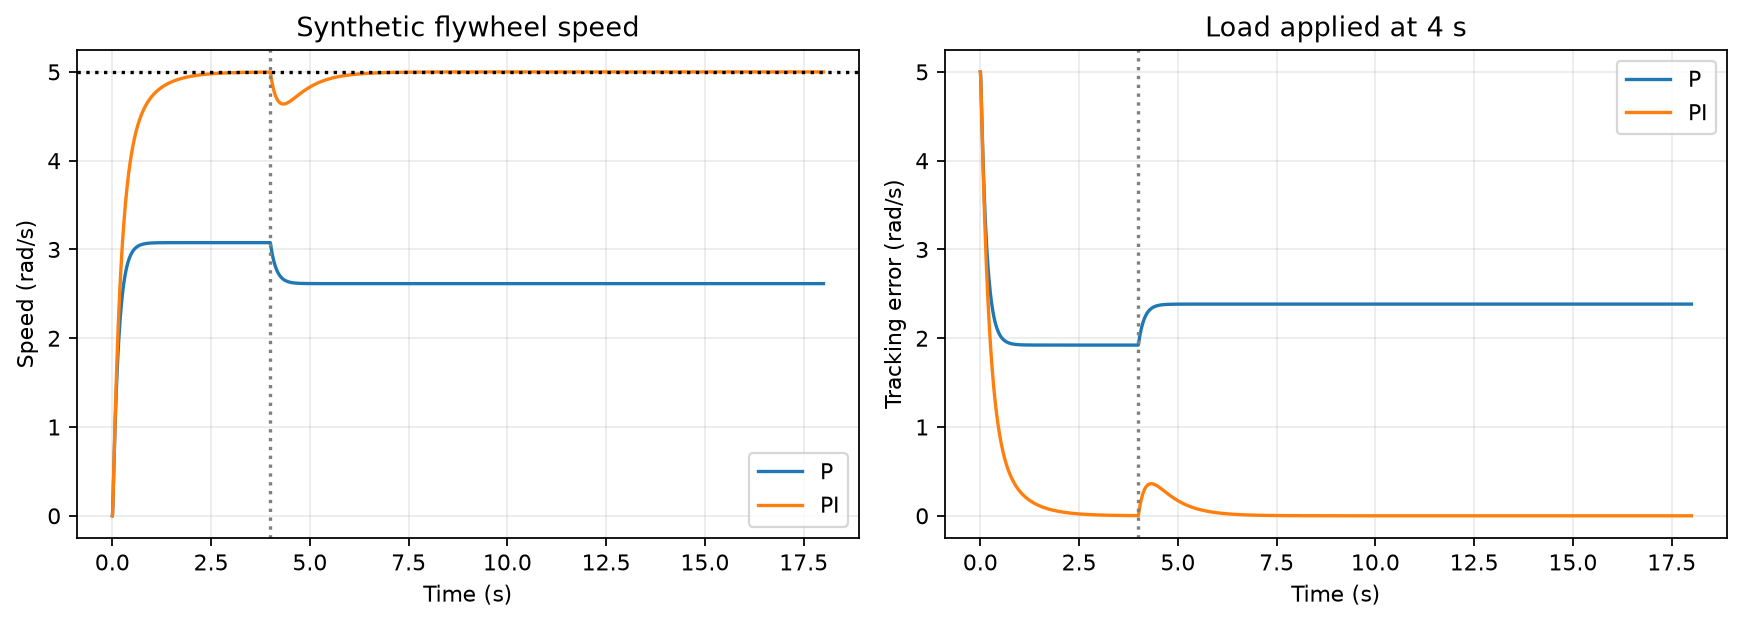
\includegraphics[width=\linewidth,height=.46\textheight,keepaspectratio]{response.png}\end{center}
\section{Method references}
The equations use standard balance laws and feedback-control methods. Further explanation: \url{https://apmonitor.com/pdc/} and \url{https://fbsbook.org/}. Implementation documentation: \url{https://python-control.readthedocs.io/en/0.10.2/}. See the repository reference catalog for individual topics and videos.
\end{document}
